A Inception-v3 iteratív tanításának eredményei négy lépésben először 1000 majd 5000 azután 10000 végül pedig 25000 képes halmazon. Ezelet a lépéseket 1k, 5k 10k 25k rövidítésekkel fogom jelölni.

%1K-----------------------------------------------------------------------------
\subsubsection{1k adathalmazon történő tanítás lépései Inception-v3 modellen.}


\subsubsection{1k adathalmazon történő tanítás grafikonja Inception-v3 modellen.}
  \begin{figure}[H]
    \centering
    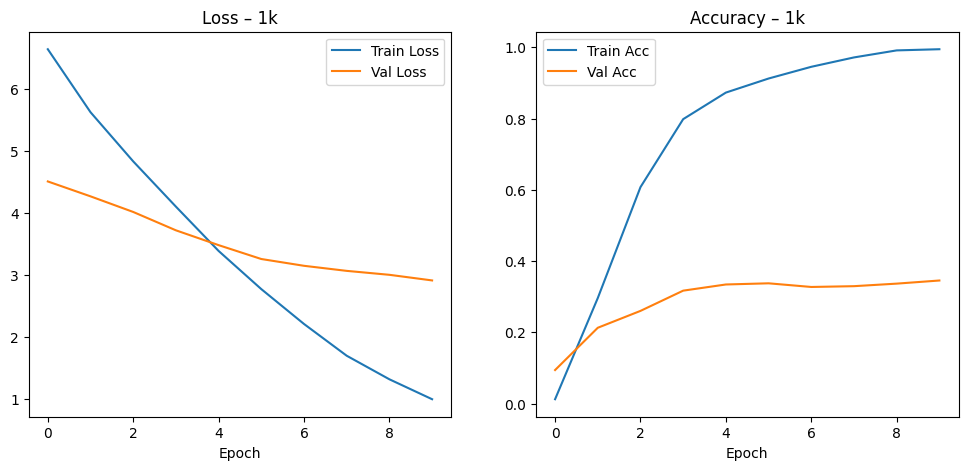
\includegraphics[width=1.0\textwidth]{images/phase03/phase03_Inception-v3_1K_learning_curve.png}
    \caption{1k adathalmazon történő tanítás grafikonja Inception-v3 modellen.}
    \label{fig:phase03_Inception-v3_1K_learning_curve}
  \end{figure}

  \subsubsection{1k adathalmazon történő tanítás eredményei.}
  \begin{center}
    \begin{longtable}{l c}
    \caption{1k tanítás Inception-v3-en.} \label{tab:phase03_Inception-v3_1k} \\
    \toprule
    \textbf{Metrika} & \textbf{Érték} \\
    \midrule
    \endfirsthead
    \toprule
    \textbf{Metrika} & \textbf{Érték} \\
    \midrule
    \endhead
    Top-1 Accuracy & 0.3022 \\
    Top-5 Accuracy & 0.6505 \\
    Precision      & 0.2851 \\
    Recall         & 0.3149 \\
    F1-score       & 0.2820 \\
    Inference time & 31.49 sec \\
    \bottomrule
    \end{longtable}
  \end{center}

%5K-----------------------------------------------------------------------------
\subsubsection{5k adathalmazon történő tanítás lépései Inception-v3 modellen.}


\subsubsection{5k adathalmazon történő tanítás grafikonja Inception-v3 modellen.}
  \begin{figure}[H]
    \centering
    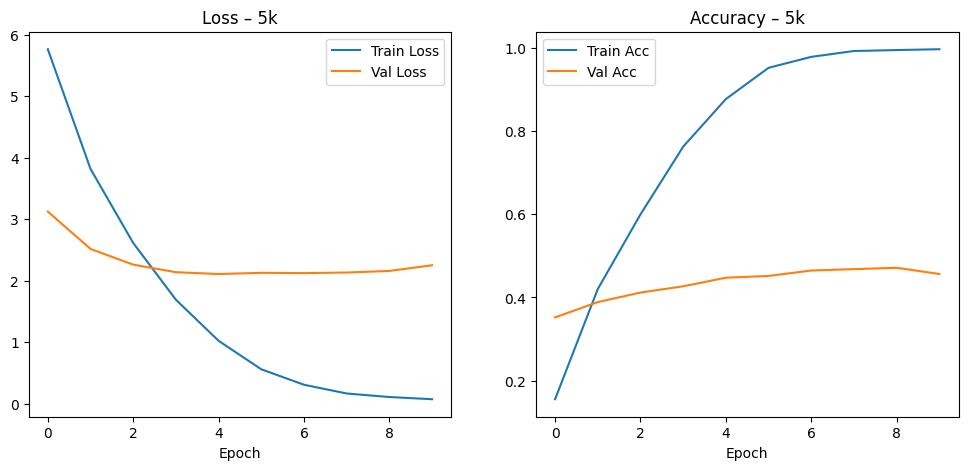
\includegraphics[width=1.0\textwidth]{images/phase03/phase03_Inception-v3_5K_learning_curve.png}
    \caption{5k adathalmazon történő tanítás grafikonja Inception-v3 modellen.}
    \label{fig:phase03_Inception-v3_5K_learning_curve}
  \end{figure}


\subsubsection{5k adathalmazon történő tanítás eredményei.}
  \begin{center}
    \begin{longtable}{l c}
    \caption{5k tanítás Inception-v3-en.} \label{tab:phase03_Inception-v3_5k} \\
    \toprule
    \textbf{Metrika} & \textbf{Érték} \\
    \midrule
    \endfirsthead
    \toprule
    \textbf{Metrika} & \textbf{Érték} \\
    \midrule
    \endhead
    Top-1 Accuracy & 0.4603 \\
    Top-5 Accuracy & 0.7766 \\
    Precision      & 0.4254 \\
    Recall         & 0.4762 \\
    F1-score       & 0.4325 \\
    Inference time & 31.72 sec \\
    \bottomrule
    \end{longtable}
  \end{center}

%10K-----------------------------------------------------------------------------
\subsubsection{10k adathalmazon történő tanítás lépései Inception-v3 modellen.}


\subsubsection{10k adathalmazon történő tanítás grafikonja Inception-v3 modellen.}
  \begin{figure}[H]
    \centering
    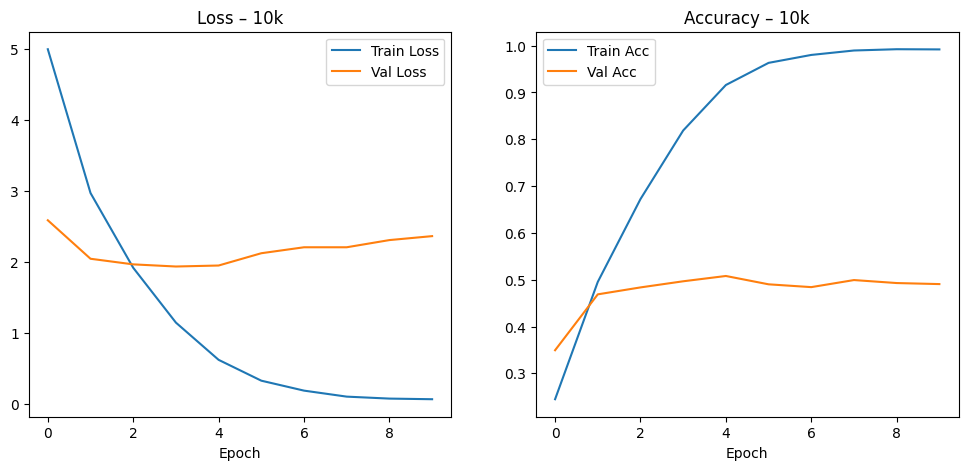
\includegraphics[width=1.0\textwidth]{images/phase03/phase03_Inception-v3_10K_learning_curve.png}
    \caption{10k adathalmazon történő tanítás grafikonja Inception-v3 modellen.}
    \label{fig:phase03_Inception-v3_10K_learning_curve}
  \end{figure}

\subsubsection{10k adathalmazon történő tanítás eredményei.}
  \begin{center}
    \begin{longtable}{l c}
    \caption{10k tanítás Inception-v3-en.} \label{tab:phase03_Inception-v3_10k} \\
    \toprule
    \textbf{Metrika} & \textbf{Érték} \\
    \midrule
    \endfirsthead
    \toprule
    \textbf{Metrika} & \textbf{Érték} \\
    \midrule
    \endhead
    Top-1 Accuracy & 0.5133 \\
    Top-5 Accuracy & 0.8177 \\
    Precision      & 0.4782 \\
    Recall         & 0.5421 \\
    F1-score       & 0.4905 \\
    Inference time & 31.71 sec \\
    \bottomrule
    \end{longtable}
  \end{center}

%25K-----------------------------------------------------------------------------
\subsubsection{25k adathalmazon történő tanítás lépései Inception-v3 modellen.}


\subsubsection{25k adathalmazon történő tanítás grafikonja Inception-v3 modellen.}
  \begin{figure}[H]
    \centering
    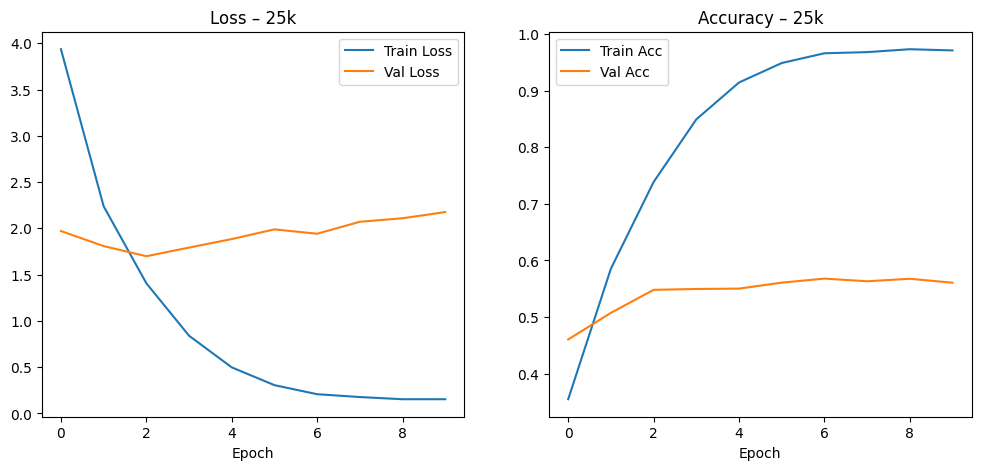
\includegraphics[width=1.0\textwidth]{images/phase03/phase03_Inception-v3_25K_learning_curve.png}
    \caption{25k adathalmazon történő tanítás grafikonja Inception-v3 modellen.}
    \label{fig:phase03_Inception-v3_25K_learning_curve}
  \end{figure}

\subsubsection{25k adathalmazon történő tanítás eredményei.}
  \begin{center}
    \begin{longtable}{l c}
    \caption{25k tanítás Inception-v3-en.} \label{tab:phase03_Inception-v3_25k} \\
    \toprule
    \textbf{Metrika} & \textbf{Érték} \\
    \midrule
    \endfirsthead
    \toprule
    \textbf{Metrika} & \textbf{Érték} \\
    \midrule
    \endhead
    Top-1 Accuracy & 0.5499 \\
    Top-5 Accuracy & 0.8376 \\
    Precision      & 0.5310 \\
    Recall         & 0.5978 \\
    F1-score       & 0.5436 \\
    Inference time & 31.82 sec \\
    \bottomrule
    \end{longtable}
  \end{center}

\subsubsection{Inception-v3 iteratív tanítás összefoglaló}
  \begin{center}
    \begin{longtable}{lllllll}
    \caption{Összehasonlító táblázat a Inception-v3 iteratív tanításáról.}\label{tab:phase3_Inception-v3_summary_table}\\
    \toprule
    Minta & Top-1 & Top-5 & Precision & Recall & F1 & Time(sec) \\
    \midrule
    \endfirsthead
    \toprule
    Minta & Top-1 & Top-5 & Precision & Recall & F1 & Time(sec) \\
    \midrule
    \endhead
    1k & 0.3022 & 0.6505 & 0.2851 & 0.3149 & 0.2820 & 31.49 \\
    5k & 0.4603 & 0.7766 & 0.4254 & 0.4762 & 0.4325 & 31.72 \\
    10k & 0.5133 & 0.8177 & 0.4782 & 0.5421 & 0.4905 & 31.71 \\
    25k & 0.5499 & 0.8376 & 0.5310 & 0.5978 & 0.5436 & 31.82 \\
    \bottomrule
    \end{longtable}
  \end{center}

  \subsubsection{Összehasonlító grafikon a Inception-v3 iteratív tanításáról.}
  \begin{figure}[H]
    \centering
    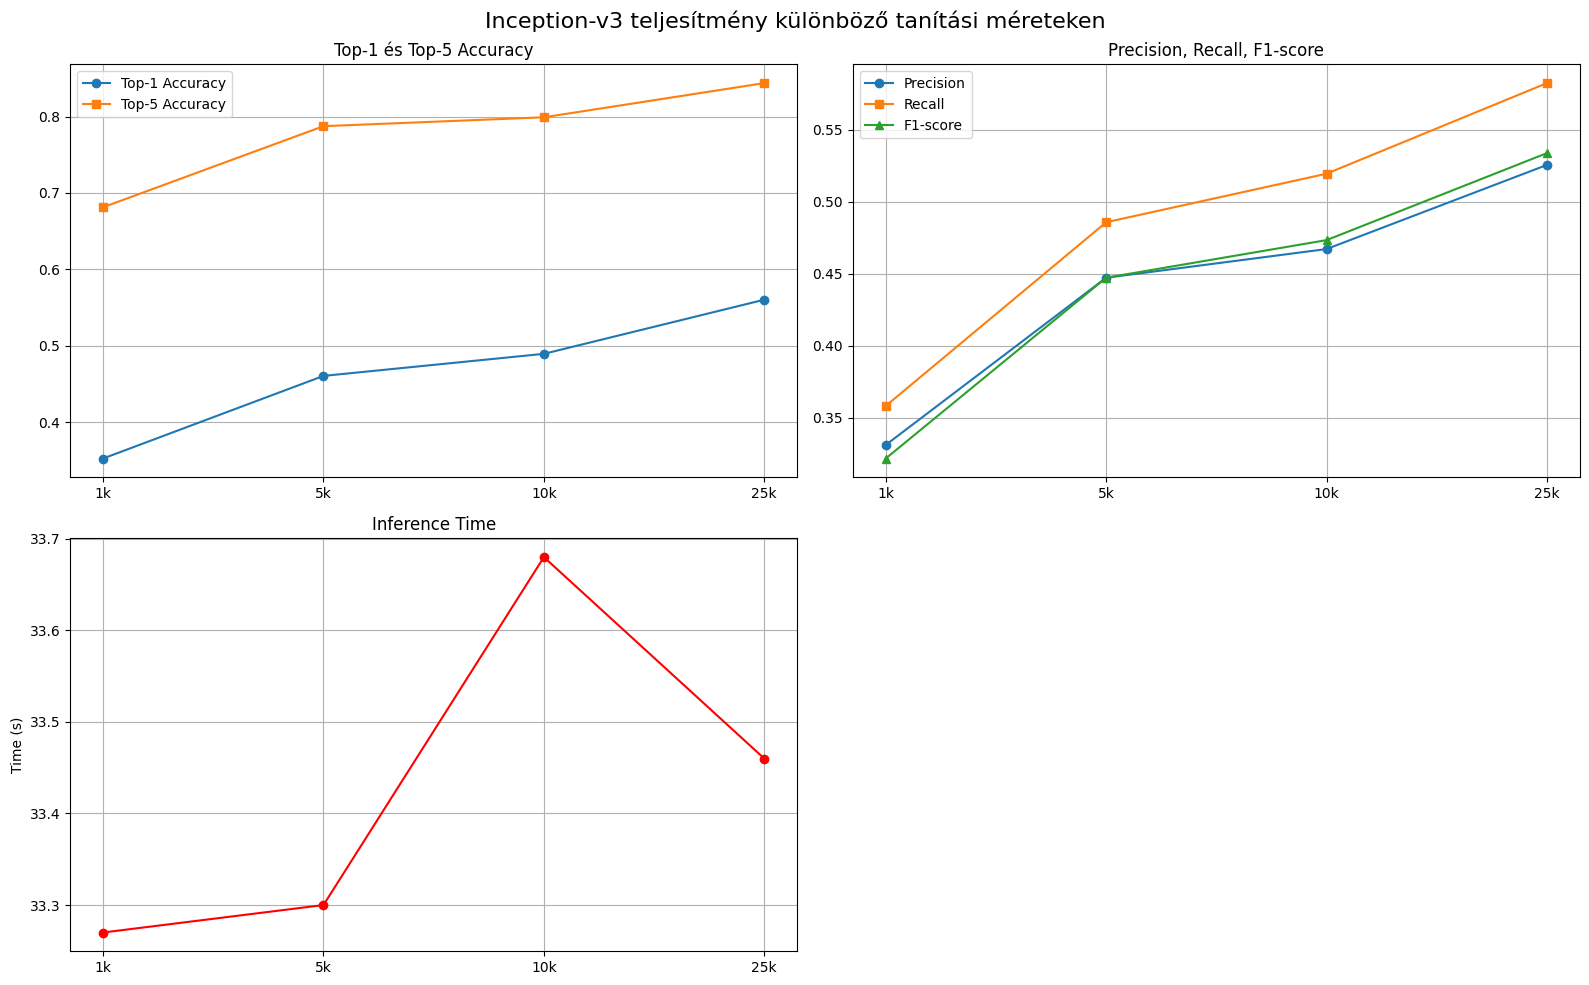
\includegraphics[width=1.0\textwidth]{images/phase03/phase03_Inception-v3_summary_curve.png}
    \caption{Összehasonlító grafikon a Inception-v3 iteratív tanításáról.}
    \label{fig:phase03_Inception-v3_summary_curve}
  \end{figure}

  \subsubsection{Összehasonlító metrika grafikon a Inception-v3 iteratív tanításáról.}
  \begin{figure}[H]
    \centering
    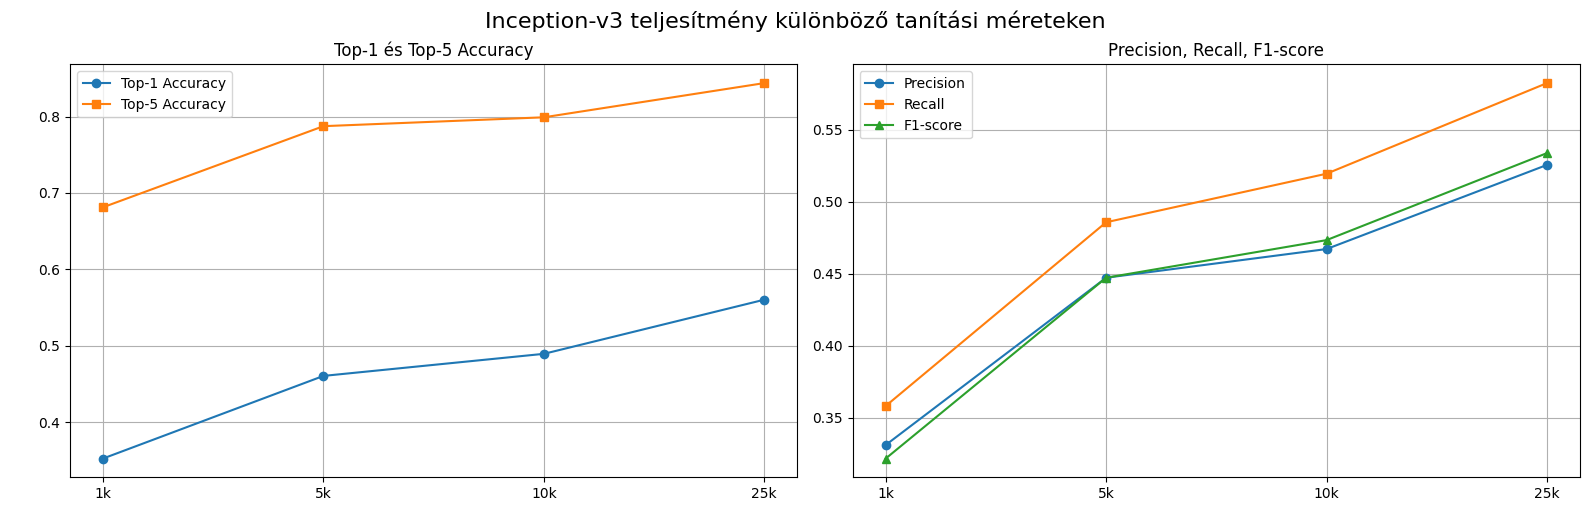
\includegraphics[width=1.0\textwidth]{images/phase03/phase03_Inception-v3_summary_curve_metrics.png}
    \caption{Összehasonlító metrika grafikon a Inception-v3 iteratív tanításáról.}
    \label{fig:phase03_Inception-v3_summary_curve_metrics}
  \end{figure}

  \subsubsection{Összehasonlító idő grafikon a Inception-v3 iteratív tanításáról.}
  \begin{figure}[H]
    \centering
    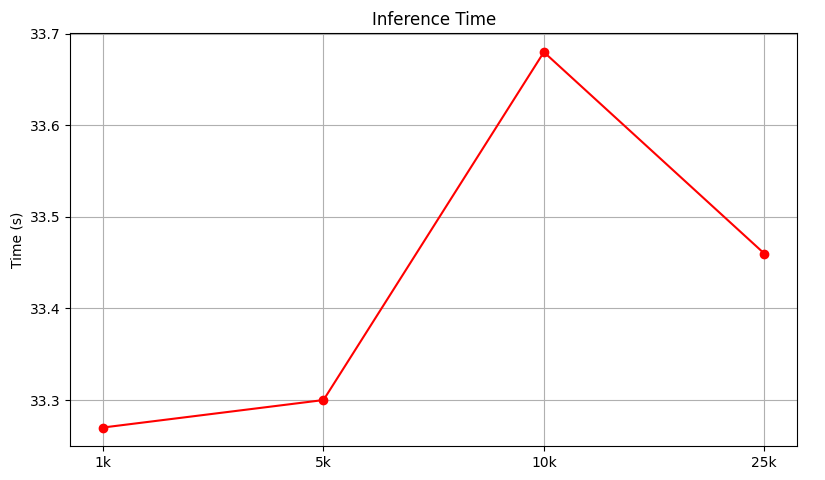
\includegraphics[width=1.0\textwidth]{images/phase03/phase03_Inception-v3_summary_curve_time.png}
    \caption{Összehasonlító idő grafikon a Inception-v3 iteratív tanításáról.}
    \label{fig:phase03_Inception-v3_summary_curve_time}
  \end{figure}

  \subsubsection{Összehasonlító grafikon a Inception-v3 iteratív tanításáról 10 EPOCH-on keresztül.}
  \begin{figure}[H]
    \centering
    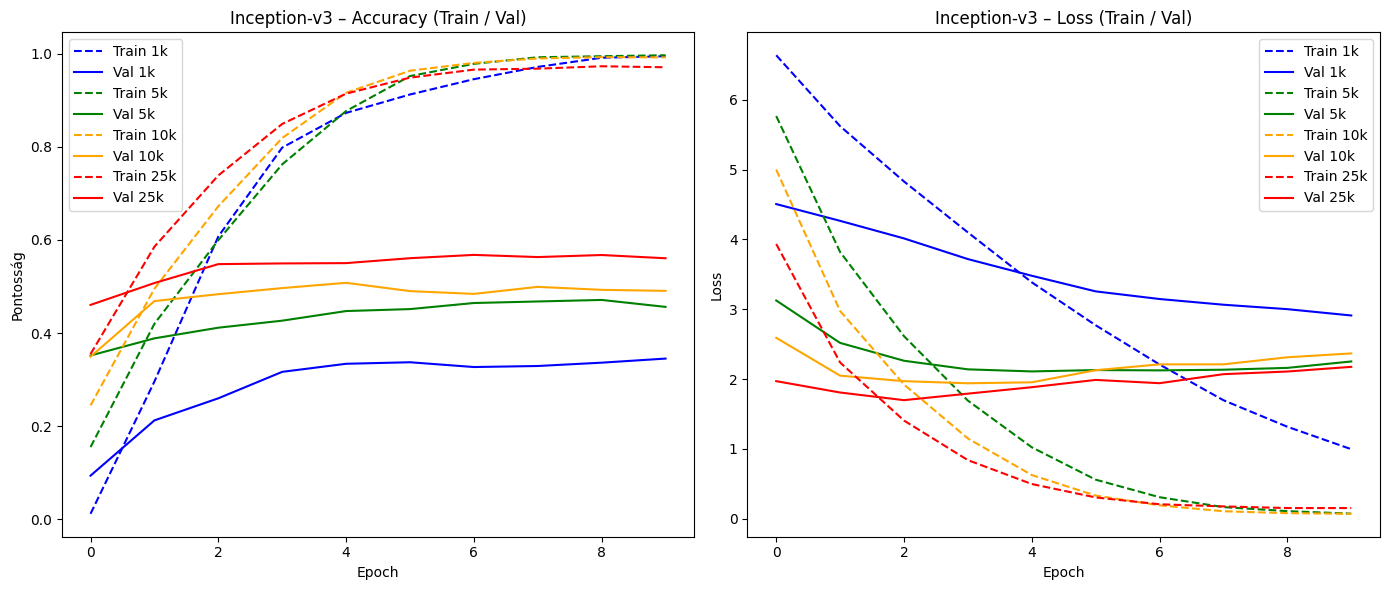
\includegraphics[width=1.0\textwidth]{images/phase03/phase03_Inception-v3_learning_summary_curve.png}
    \caption{Összehasonlító grafikon a Inception-v3 iteratív tanításáról 10 EPOCH-on keresztül.}
    \label{fig:phase03_Inception-v3_learning_summary_curve}
  \end{figure}

  \subsubsection{Összehasonlító Confusion Matrix a Inception-v3 iteratív tanításáról.}
  \begin{figure}[H]
    \centering
    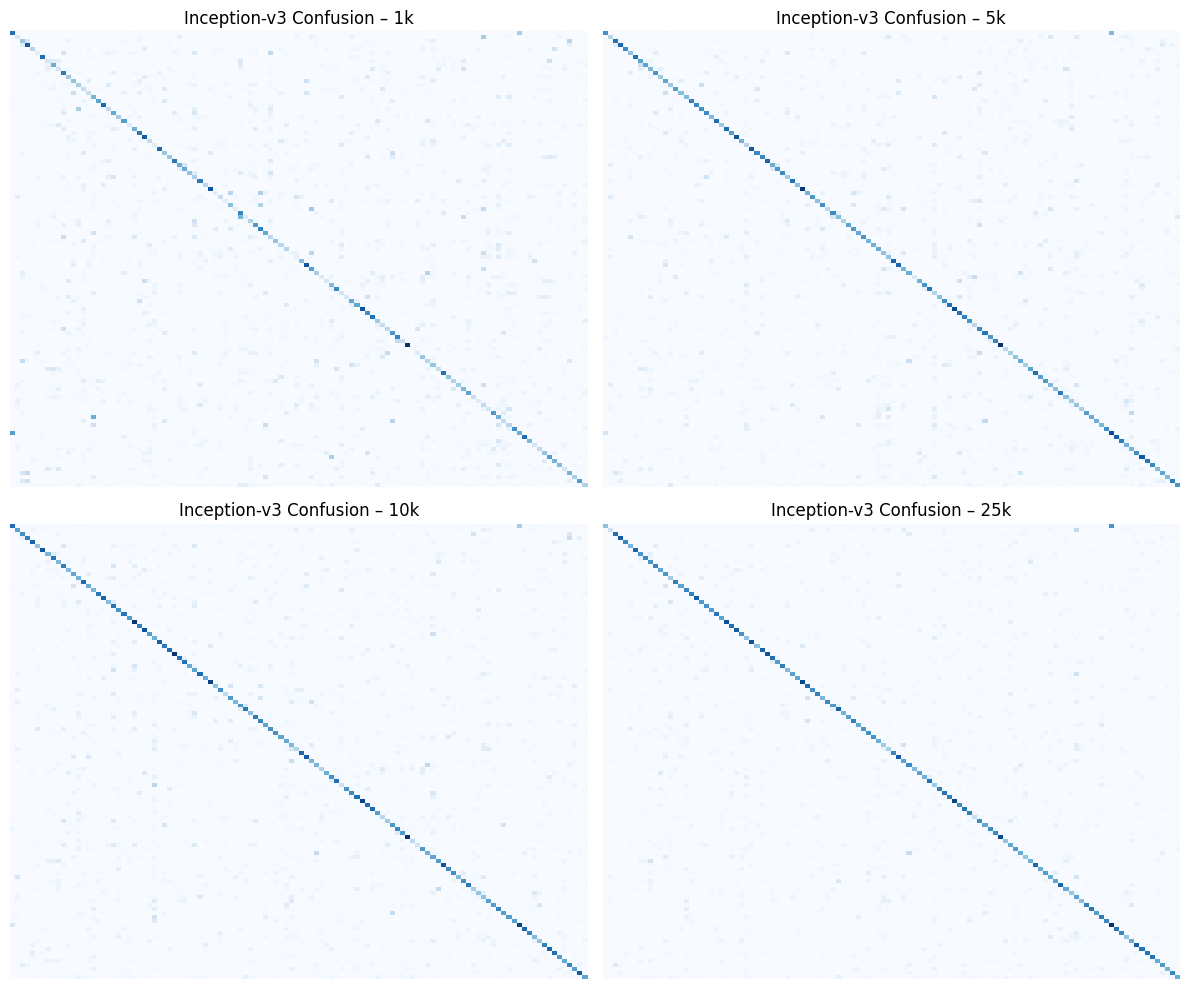
\includegraphics[width=1.0\textwidth]{images/phase03/phase03_Inception-v3_Confusion_Matrix_summary_curve.png}
    \caption{Összehasonlító Confusion Matrix a Inception-v3 iteratív tanításáról 10 EPOCH-on keresztül.}
    \label{fig:phase03_Inception-v3_Confusion_Matrix_summary_curve}
  \end{figure}